\documentclass{knowdive}
\usepackage{color,soul}
\usepackage{subcaption}
\usepackage{fancyhdr}
\usepackage{lastpage}
\usepackage{textcomp}
\usepackage{lscape}
\usepackage{rotating}
\usepackage{multirow}
\usepackage{listings}
\usepackage[table,xcdraw]{xcolor}
\usepackage{amsmath}
\usepackage{graphicx}
\usepackage{enumerate}
\usepackage{hyperref}
\usepackage{rotating}
\graphicspath{ {images/} }

\usepackage{titlesec}
\titleformat{\section}{\LARGE\bfseries}{\thesection}{1em}{}

\usepackage{array, makecell}
%\hypersetup{
	%pdfauthor={Author1, \and Author2},
	%pdftitle={Collectives.State of the Art},
       %pdfkeywords = {},
      %pdfsubject={}
      %}
%\usepackage{hyperref}


\graphicspath{ {images/} }
\usepackage{comment}

\title{KG 2025 - Project Report Template}

\author{Author1, ..., AuthorN}

\revisionhistory{
    \revision{1}{\today}{Mayukh Bagchi}{Document created}
}
\newpage

\fancypagestyle{plain}{
  \fancyhf{}% Clear header/footer
  %\fancyhead[R]{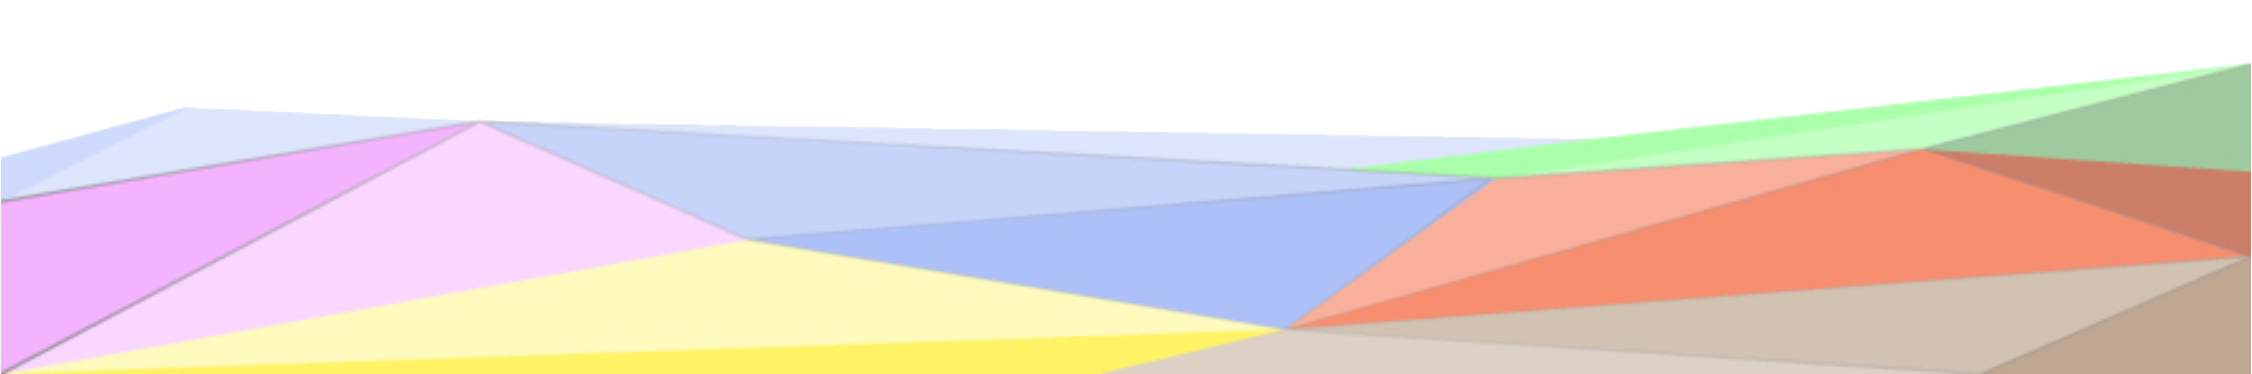
\includegraphics[width=1.0\linewidth,height=5pt]{Knowdive_color_bar}}% Right header
  \fancyfoot[L]{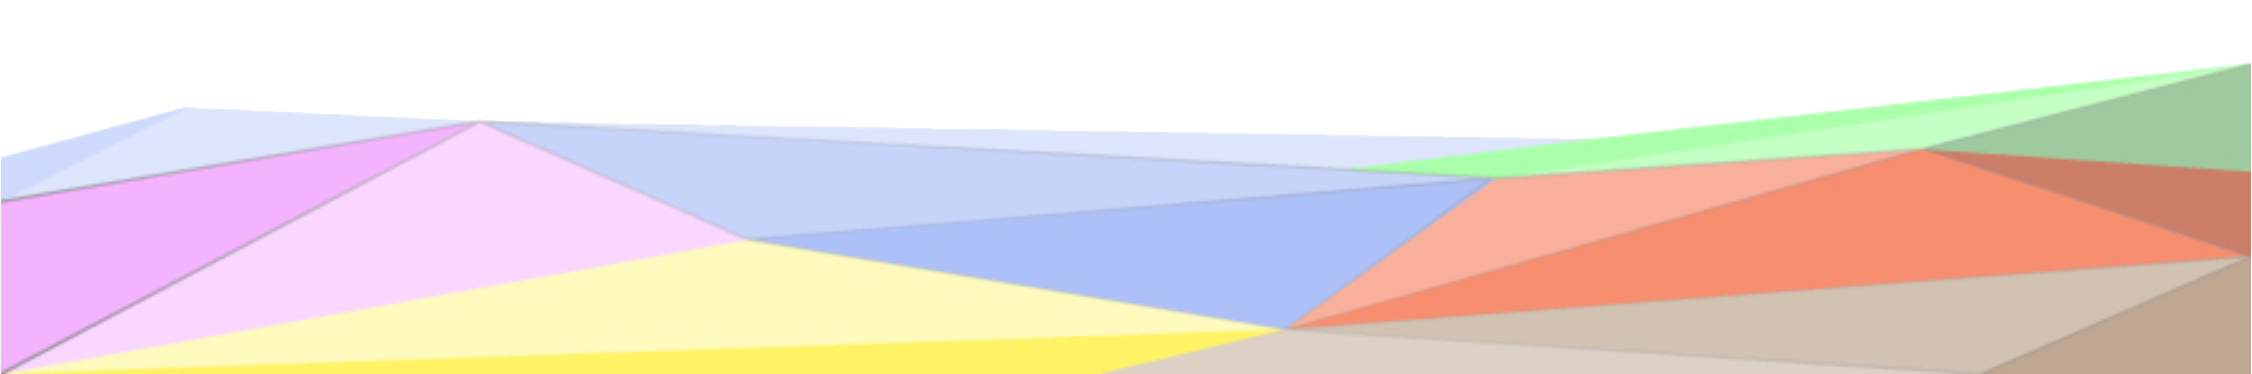
\includegraphics[width=1.0\linewidth,height=45pt]{Knowdive_color_bar}}% Left footer
  \fancyfoot[C]{Page \thepage\  / \pageref{LastPage}}
}

\pagestyle{plain}
%\makeglossaries
%input{glossaries}
\begin{document}
\maketitle
\begin{sloppypar}
\large
\begin{spacing}{1.05}
%\gls{latex}
%\gls{batex}
%\gls{eType}
%\printglossary

\section{Introduction}
Reusability is one of the main principles in the Knowledge Graph (KG) development process defined by iTelos. The KG project documentation plays an important to enhance the reusabiltiy of the resources handled and produced during the process. A clear description of the resources, the process (and sub processes) developed and evaluation at each step of the process provides a clear understanding of the project, thus serving such an information to external readers for the future exploitations of the project's outcomes.\\

\noindent The current document aims to provide a detailed report of the project developed following the iTelos methodology. The report is structured, to describe:
\begin{itemize}
    \item Section 2: Definition of the project's purpose and related information gathering.
    
    \item Sections 3, 4, 5, 6: The description of the iTelos process phases and their activities, divided by knowledge and data layer activities, as well as the evaluation of the resources produced in terms of fit for the chosen purpose.

    \item Section 7: The description of the metadata produced for all (and all kind of) the resources handled and generated by the iTelos process, while executing the project.

    \item Section 8: Conclusion and open issues summary.
\end{itemize}

\section{Project Design}

This section has to report and describe:
\begin{itemize}
    \item The \textbf{broad definition} of the KG project's Domain of Interest, by defining its boundaries in space and time. The definition of the domain of interest is crucial to set the space and time boundaries of the project purpose. The domain of interest description informs the reader about the geographical space, as well as the period of time, in which the project purpose is considered. 

    \item The \textbf{broad definition} of the KG project's general purpose, by reporting the main purpose as expressed by the final user. The description of the purpose in this section is an "informal" description, meaning by this that it is expressed by using a natural language paragraph, which need to be exploited, have not yet been identified. 

\end{itemize}
\section{Purpose Definition}
The iTelos methodology proposes a systematic approach designed to simplify and reduce the effort required to build Knowledge Graphs (KGs), focusing on the specific purpose indicated by the end user. This section provides a detailed overview of the first phase of the methodology.

\subsection{Purpose Formalization}
In this phase, the informal purpose is structured and formalized to guide the development of the Knowledge Graph. Purpose formalization includes the specification of the Domain of Interest, the identification of the main concepts (Concept Identification), the definition of usage scenarios and personas, the formulation of the Competency Questions (CQs) that the Knowledge Graph must be able to answer, and the definition of the conceptual model (ER Model Definition). This step ensures that the design of the KG is aligned with user requirements and provides a clear and consistent framework for the subsequent modeling and implementation phases.
\subsubsection{Informal Purpose}
The purpose of this project is to build a Knowledge Graph (KG) that models the meteorological facilities in the territory and, consequently, the climate and potential climate change in Trentino. The KG will organize information in a structured and accessible way, allowing it to answer precise user queries, such as identifying the locations of weather stations, analyzing temperature and rainfall over recent years, pinpointing areas with the highest temperature increases, and detecting signs of climate change based on historical data.

\subsubsection{Domain of Interest}
The Domain of Interest (DoI) for this project is the Trentino region in 2025, with a particular focus on meteorological phenomena and climate change. The Trentino region exhibits a wide variety of microclimates and weather conditions, ranging from high alpine areas to valleys and lakes, making it an ideal natural laboratory for climate study. The project’s geographic scope covers the entire region, including weather stations, climate sensors, and historical data, enabling a comprehensive analysis of climate patterns.\\
Key features of the domain include:
\begin{itemize}
    \item \textit{Meteorological Monitoring}: Data on temperature, precipitation, humidity, wind, and other variables measured by weather stations distributed throughout the territory.
    \item \textit{Climate Change Monitoring}: Analysis of historical trends and detection of climate variation signals, such as increases in average temperature, changes in precipitation patterns, and local climatic anomalies.
\end{itemize}


\subsubsection{Scenario}
This section presents several usage scenarios, describing the different aspects considered by the project’s purpose.
\begin{itemize}
    \item \textbf{Maria} and her boyfriend, two local researchers, are analyzing precipitation trends in Trentino over the past ten years. They want to identify areas where rainfall has significantly increased or decreased to understand potential impacts on agricultural and forested areas. They use the Knowledge Graph to retrieve historical data from multiple weather stations and compare time series.
    \item \textbf{Giulia}, a climatology student, wants to study the microclimates present in the different valleys of Trentino. She needs access to temperature, humidity, and wind data collected by sensors across the territory to analyze climate variations between alpine and lake areas.
    \item \textbf{Alessandro}, responsible for civil protection, is monitoring climatic anomalies in real time. He aims to quickly identify areas with unusual temperatures or precipitation to plan preventive interventions against landslides or hydrogeological risks.
    \item \textbf{Francesca} and her group of students want to study the impact of climate change on the seasons in Trentino. They need to compare historical data with current measurements to understand the evolution of climatic phenomena, such as delayed snowfall or increased heatwaves.
    \item \textbf{Marco}, a weather enthusiast, uses the Knowledge Graph to explore long-term trends in temperature and precipitation, identify areas with the highest temperature increases, and better understand the signals of climate change in the Trentino region.
\end{itemize}

\subsubsection{Personas}
This section defines a set of real users acting within the previously described scenarios.
\begin{itemize}
    \item \textbf{Maria Bianchi}, 35 years old, a local researcher passionate about meteorology. She is interested in analyzing precipitation trends and the impact of climate change on the territory.
    \item \textbf{Giulia Ferrari}, 23 years old, a climatology student. She enjoys studying microclimates and climate variations between alpine and lake areas.
    \item \textbf{Alessandro Rossi}, 40 years old, responsible for civil protection. He monitors climatic anomalies in real time to prevent landslides and hydrogeological risks.
    \item \textbf{Francesca Romano}, 22 years old, an Erasmus student. She is interested in comparing historical and current data to study the evolution of seasonal climate phenomena.
    \item \textbf{Marco Ricci}, 28 years old, a weather enthusiast. He likes exploring long-term temperature and precipitation trends to better understand the signals of climate change in the Trentino region
\end{itemize}



\subsubsection{Competency Questions (CQs)}
\begin{tabular}{|p{5cm}|p{1cm}|p{10cm}|}
\hline
\textbf{Person} & \textbf{N.o.} & \textbf{Competency Question (CQ)} \\
\hline
Maria Bianchi & 1.1 & Which areas of Trentino have experienced significant increase in annual rainfall over the past decade? \\ Maria Bianchi & 1.2 & Which areas have shown a consistent decrease in precipitation over the past decade? \\ Maria Bianchi & 1.3 & How has the average monthly rainfall evolved in each valley or municipality of Trentino over the last ten years? \\ Maria Bianchi & 1.4 & Are there correlations between changes in rainfall and altitude or proximity to forests and agricultural land?\\ Maria Bianchi & 1.5 & Which weather stations have the most complete historical data on precipitation in Trentino? \\
\hline
Giulia Ferrari & 2.1 & What are the typical temperature ranges and humidity levels in alphine valleys compared to lake areas? \\ Giulia Ferrari & 2.2 & Which areas show microclimatic differences despite geographical proximity? \\ Giulia Ferrari & 2.3 & How does wind speed and direction vary between the Adige Valley and surrounding mountains areas? \\ Giulia Ferrari & 2.4 & Are there correlations between altitude and average annual temperature or humidity? \\ Giulia Ferrari & 2.5 & How stable are microclimates across seasons (winter vs. summer) in different valleys? \\ Giulia Ferrari & 2.6 & Which valleys show the most distinctive microclimatic patterns according to sensor data? \\
\hline
Alessandro Rossi & 3.1 & Which areas of Trentino are currently showing unusually high or low temperatures compared to historical averages? \\ Alessandro Rossi & 3.2 & Are there real-time alerts for abnormal precipitation or snowmelt that could indicate flood risks? \\ Alessandro Rossi & 3.3 & Which zones are currently under potential hydrogeological risk due to recent heavy rainfall? \\ Alessandro Rossi & 3.4 & How do current weather anomalies compare to past extreme events recorded in the KG? \\ Alessandro Rossi & 3.5 & Can the KG highlight areas with recurring climatic anomalies over multiple years? \\ Alessandro Rossi & 3.6 & Which meteorological stations are currently reporting anomalies in temperature or precipitation beyond expected thresholds?\\
\hline
Francesca Romano & 4.1 & How have the average start and end dates of each season changed in Trentino over the past 30 years?\\ Francesca Romano & 4.2 & Has the timing or duration of snowfall periods shifted over time? \\ Francesca Romano & 4.3 & Are heat waves occurring more frequently or lasting longer than in the past? \\ 
\hline
\end{tabular}
\begin{tabular}{|p{5cm}|p{1cm}|p{10cm}|}
\hline
Francesca Romano & 4.4 & How does current spring temperature compare to historical averages from the 1980s and 1990s? \\ Francesca Romano & 4.5 & Which areas show the most significant seasonal shifts (e.g., warmer winters, delayed autumn)? \\ Francesca Romano & 4.6 & How has average precipitation in summer and winter evolved over time?\\
\hline
Marco Ricci & 5.1 & Which areas of Trentino gave recorder the highest temperature increases over the past 50 years? \\ Marco Ricci & 5.2 & How have long-term temperature and precipitation trends evolved across different valleys? \\ Marco Ricci & 5.3 & What are the clearest signals of climate change (e.g., rising temperatures, changing rainfall patterns) in the KG data? \\ Marco Ricci & 5.4 & Are there locations showing evidence of both increased temperature and decreased precipitation? \\ Marco Ricci & 5.5 & Can the KG visualize how average annual temperatures have evolved decade by decade? \\ Marco Ricci & 5.6 & Which weather stations show the most evident long-term warming trends? \\
\hline
\end{tabular}
\subsubsection{Concept Identification}

\subsubsection{ER model definition}
\subsubsection{Report}






\subsection{Information Gathering}
This sub-section aims at reporting the execution of the activities involved in Information Gathering. The report, starting from the current section, is organized along two main dimensions. The information gathering sub activities are:
\begin{itemize}
    \item \textbf{KG/KnowDive Data Sources}: these activities aim at collecting the already available KG/KnowDive resources considered for the project. More in detail the resources here described, are "quality and formal" resources (compliant with the quality and reusability guidelines defined by iTleos) which need minimal processing or don't need to be processed or created. The resources described in this section are those that can be already considered to satisfy the project's purpose.
    \begin{itemize}
        \item Knowledge layer:
        \begin{itemize}
            \item Sources description
            \item Formal resources collection;
            \item Formal resources classification over common, core and contextual
        \end{itemize}
        \item Data layer:
        \begin{itemize}
            \item Sources description
            \item Formal resources collection;
            \item Formal resources classification over common, core and contextual
        \end{itemize}
    \end{itemize}

    \item \textbf{External Data Sources}: these activities aim at collecting "informal" resources from sources with a higher level of heterogeneity. The resources collected by the producer process are not necessarily compliant with the iTelos quality and reusability guidelines. Those are the resources that the KG team will transform into quality resources at the end of the process.
    \begin{itemize}
        \item Knowledge layer:
        \begin{itemize}
            \item Sources description
            \item Informal resources collection and scraping;
            \item Informal resources classification over common, core and contextual
        \end{itemize}
        \item Data layer:
        \begin{itemize}
            \item Sources description
            \item Resources collection and scraping;
            \item Resources classification over common, core and contextual
        \end{itemize}
    \end{itemize}
\end{itemize}

\noindent The report of the work done during the above activities of the methodology, has to includes also the description of the  different choices made, with their strong and weak points. In other words the report should provide to the reader, a clear description of the reasoning conducted by all the different team members.


Evaluation - Purpose Definition: A detailed description of the purpose layer evaluation:
\begin{itemize}
    \item Given the data sources gathered - How many scenarios initially considered? How many scenarios finally considered? report each scenario-level details in a table.
    \item Given the data sources gathered - How many users initially considered? How many users finally considered? report each user-level details in a table.
    \item Given the data sources gathered - How many CQs initially considered? How many CQs finally considered? report each CQ-level details in a table.
    \item If valid, report dataset-level formatting and transformations done in this phase?
\end{itemize}
\section{Language Definition}

This section is dedicated to the description of the Language Definition phase. Like in the previous section, it aims to describe the different sub activities performed by all the team members, as well as the phase outcomes produced. The language definition sub activities include:
\begin{itemize}
    \item The activities aim at fixing the language (concepts and words for etype, object property and data property) used to represent the information required to satisfy the project purpose. With this objective, the knowledge ad data resources are handled in this phase following the below activities:
    \begin{itemize}
        \item Knowledge layer:
        \begin{itemize}
            \item Fixing Language Terms: finalize the informal terms for - etype, object property and data property - considered in the purpose definition phase.
            \item Language Teleontology alignment: Given the already provided Language Teleontology, align each language term to a parent lexical-semantic concept in the Language Teleontology. In case, there is no parent concept, enrich and align the Language Teleontology with your purpose-specific terms.
        \end{itemize}
        \item Data layer:
        \begin{itemize}
            \item Dataset filtering/cleaning/formatting.
        \end{itemize}
    \end{itemize}
\end{itemize}

\noindent The report of the work done during this phase of the methodology, has to includes also the description of the  different choices made, with their strong and weak points. In other words the report should provide to the reader, a clear description of the reasoning conducted by all the different team members.

Evaluation - Language Definition: A detailed description of the Language layer evaluation over the language layer of the KG -
\begin{itemize}
    \item How many etypes terms initially considered? How many etypes terms finally considered? How many etypes terms could be aligned to the  language teleontology? report each etype term level details in a table.
    \item How many object property terms initially considered? How many object property terms finally considered?  How many object property terms could be aligned to the  language teleontology? report each object property term level details in a table.
    \item How many data property terms initially considered? How many data property terms finally considered?  How many data property terms could be aligned to the language teleontology? report each data property term level details in a table.
    \item If valid, how was the language teleontology enriched/adapted? report element level details in a table.
    \item Did you have to return to change something in the Purpose Definition phase? If yes, report here.
    \item If valid, report dataset-level formatting and transformations done in this phase?
\end{itemize}

\section{Knowledge Definition}
This section is dedicated to the description of the Knowledge Definition phase. Like in the previous section, it aims to describe the different sub activities performed by all the team members, as well as the phase outcomes produced. The knowledge definition sub activities include:
\begin{itemize}
    \item The activities aim at defining the knowledge structure of the information, using the language terms, to be considered to satisfy the project purpose. More in details, the producer process, in this phase, aims at defining the knowledge structure for each dataset to be formalize, singularly. The data within such datasets, are then aligned with the structure d knowledge.
    
    \begin{itemize}
        \item Knowledge layer:
        \begin{itemize}
            \item Teleology definition: You are provided with fragments of ontologies. You need to compose relevant fragments together to model the Teleology. Notice, in very specific aspects of your purpose, you might have to enrich the ontology fragments or, in extreme cases, create the fragment from scratch.
            \item Knowledge Teleontology alignment: given the teleology, align the etype, object properties and data properties to their parents in the provided Knowledge Teleontology. In specific cases of your purpose, you might need to enrich and extend the Knowledge Teleontology with free etypes and free properties.
        \end{itemize}
        \item Data layer:
        \begin{itemize}
            \item Dataset cleaning and formatting following the shape (etype, object properties and data properties) of the knowledge layer.
        \end{itemize}
    \end{itemize}
\end{itemize}

\noindent The report of the work done during this phase of the methodology, has to includes also the description of the  different choices made, with their strong and weak points. In other words the report should provide to the reader, a clear description of the reasoning conducted by all the different team members.

Evaluation - Knowledge Definition: A detailed description of the Knowledge layer evaluation over the knowledge layer of the KG -
\begin{itemize}
    \item How many etypes initially considered? How many etypes finally considered? How many etypes composed from the provided reference ontology fragments for modelling the Teleology? How many etypes could be aligned to the  knowledge teleontology? report each etype level details in a table.
    \item How many object properties initially considered in the teleology? How many object properties finally considered? How many object properties could be aligned to the knowledge teleontology? report each object property details in a table.
    \item How many data properties initially considered in the teleology? How many data properties finally considered?  How many data property could be aligned to the knowledge teleontology? report each data property term details in a table.
    \item If valid, how was the knowledge teleontology enriched/adapted? report element level details in a table.
    \item Did you have to return to change something in the Purpose Definition and/or Language Definition phase? If yes, report here.
    \item If valid, report dataset-level formatting and transformations done in this phase?
\end{itemize}
\section{Entity Definition}
This section is dedicated to the description of the Entity Definition phase. Like in the previous section, it aims to describe the different sub activities performed by all the team members, as well as the phase outcomes produced. The division between knowledge and data activities in this section is not defined, because, in this phase the two layers are merged to form a single data structure composed by the knowledge structures defined in the last section, and the aligned dataset. The obtained result is a structured Knowledge Graph including both the two layers.


\noindent Entity Definition sub activities:
\begin{itemize}
    \item the first set of activities aim at merging the knowledge layer of a single dataset with the data values present within such a dataset.
    
    \begin{itemize}
            \item Entity identification 
            \item Data mapping
    \end{itemize}

    \item the second set of activities merges the knowledge and data layers considering the composition of different datasets, thus mapping multiple datasets to one single knowledge structure (the teleontology), instead of merging the mapping one dataset to its relative knowledge structure, as the producer process does.
    
    \begin{itemize}
            \item Entity identification 
            \item Data mapping
    \end{itemize}
\end{itemize}

\noindent The report of the work done during this phase of the methodology, has to includes also the description of the  different choices made, with their strong and weak points. In other words the report should provide to the reader, a clear description of the reasoning conducted by all the different team members.

Evaluation - Entity Definition: A detailed description of the Entity layer evaluation over the data layer of the KG -
\begin{itemize}
    \item How many entities initially considered? How many entities finally considered? How many entities could be modelled as the KG?
    \item If valid, how was the knowledge graph enriched/adapted over different iterations of Karma mapping? report details in a table.
    \item Other details/ difficulties encountered during Entity Definition via Karma.
    \item Did you have to return to change something in the Purpose Definition and/or Language Definition and/or Knowledge Definition phase? If yes, report here.
    \item If valid, report dataset-level formatting and transformations done in this phase?
\end{itemize}
\section{Evaluation}

This section aims at describing the evaluation performed at the end of the whole process over the final outcome of the iTelos methodology. More in details, this section as to report:

\begin{itemize}
    \item the final Knowledge Graph information statistics (like, number of etypes and properties, number of entities for each etype, and so on).
    \item Knowledge layer evaluation: the results of the application of the evaluation metrics applied over the knowledge layer of the final KG.
    \item Data layer evaluation: the results of the application of the evaluation metrics applied over the data layer of the final KG.
    \item Query execution: the description of the competency queries executed over the final KG in order to test the suitability of the KG to satisfy the project purpose. How many CQs could be transformed into SPAQRL queries? For how many SPARQL queries the KG returned desired answers?
\end{itemize}


\section{Metadata Definition}

In this section the report collects the definitions of all the metadata defined for the different resources produced along the whole process. The metadata defined in this phase describes both the final outcome of the project, and the intermediate outcome of each phase.\\

\noindent The definition of the metadata, is crucial to enable the distribution (sharing) of the resource produced. For this reason it is important to describe also where such metadata will be published to distribute the resources it describes. \\

\noindent In particular the structure of this section is organized as follows, with the objective to describe the metadata relative to all the type of resources produced by the project.\\
\begin{itemize}
    \item Language resources metadata description
    \item Knowledge resources metadata description
    \item Data resources metadata description
    \item KG metadata description
\end{itemize}



\section{Open Issues}

This section concludes the current document with final conclusions regarding the quality of the process and final outcome, and the description of the issues that (for lack of time or any other cause) remained open.\\

\begin{itemize}
    \item Did the project respect the scheduling expected in the beginning ?
    \item Are the final results able to satisfy the initial Purpose ?
        \begin{itemize}
            \item If no, or not entirely, why ? which parts of the Purpose have not been covered ?
        \end{itemize}
\end{itemize}


\noindent Moreover, this section aims to summarize the most relevant issues/problems remained open along the iTelos process. The description of open issues has to provide a clear explanation about the problems, the approaches adopted while trying to solve them and, eventually, any proposed solution that has not been applied.\\

\begin{itemize}
    \item which are the issues remained open at the end of the project ?
\end{itemize}

\end{spacing}
\end{sloppypar}
\end{document} 